\documentclass[10pt,conference,compsocconf]{IEEEtran}

% Language
%
\usepackage[english]{babel}
\usepackage[utf8]{inputenc}
\usepackage[T1]{fontenc}
\usepackage{hyphenat}
\usepackage{subfig}
\usepackage{float}
\usepackage{graphicx}
\usepackage{listings}

% Misc
%
\usepackage{xspace}
\usepackage{url}

% New commands
%
\newcommand{\ecopetrol}{\textsf{ECOPETROL}\xspace}
\newcommand\fig[1]{\textsc{figure}~\ref{#1}}
\newcommand\Fig[1]{\textsc{Figure}~\ref{#1}}

% Main
%
\begin{document}

\title{A substation automation system for the \ecopetrol power plants at Cantagallo and Yariguí}

\author{%
\IEEEauthorblockN{Jose David Tascón Vidarte}
\IEEEauthorblockA{Gers S.A.\\ \url{jose.tascon@gers.com.co}}
\and
\IEEEauthorblockN{Héctor Fabio Flórez Londoño}
\IEEEauthorblockA{Gers S.A.\\ \url{hector.florez@gers.com.co}}
\and
\IEEEauthorblockN{Juan Diego Tascón Vidarte}
\IEEEauthorblockA{Gers S.A.\\ \url{juan.tascon@gers.com.co}}
}

\maketitle

%%-*-latex-*-

\begin{abstract}
  The following paper shows the birth and development of a
  distributed automation system at the Cantagallo and Yariguí
  electrical generation centers. An architecture based on MODBUS
  at the I/O devices layer and an Ethernet network as core for the
  communications is proposed. It is important to highlight that the
  Cantagallo center is operated remotely. System integration is
  implemented by a Vijeo Citect SCADA, there, the use of the several
  Modbus protocol versions is predominant at the generation centers
  hardware. It also shows the software involving the Quantum PLC
  programming, the HMI application and the SCADA which will be the
  main automation component. Currently the application is successfully
  working at the two ECOPETROL generation centers.
\end{abstract}



%The following paper shows the birth and development of a distributed automation system at the Cantagallo and Yariguí electrical generation centers. An architecture based on MODBUS at the I/O devices layer and an Ethernet network as core for the communications is proposed. It is important to highlight that the Cantagallo center is operated remotely. System integration is implemented by a Vijeo Citect SCADA, there, the use of the several Modbus protocol versions is predominant at the generation centers hardware. It also shows the software involving the Quantum PLC programming, the HMI application and the SCADA which will be the main automation component. Currently the application is successfully working at the two ECOPETROL generation centers.


\begin{IEEEkeywords}
Substation automation system, power plant, industrial communication networks, distributed control systems
\end{IEEEkeywords}

\IEEEpeerreviewmaketitle

%%-*-latex-*-

\section{Introduction}

%TODO: poner las referencias

Because of their geographical location it is necessary to remotely
monitor the electrical substations. It is of vital importance the
automation and centralized control, thus modernizing the facilities.
The results would be a higher efficiency and a higher service
availability.

%~\cite{Kahney:1983}

Ethernet protocol has been incredibly spread into IEDs (Intelligent 
Electronic Devices) at the Substation Automation Systems (SAS).
In such scenarios, Ethernet is the leading technology for its reliability
and integrability~\cite{pozzuoli:2003}. On modern automation 
implementations it has reach the point to be used for execution of 
real-time applications~\cite{bello:2001}. Control hardware including 
PLC, smart transducers and communication equipment such as gateways 
include, most of the time, an Ethernet communication port with an option 
to use either TCP/IP or UDP~\cite{viegas:2006}. For these reasons
this technology can not be overlooked as network base and main core
for an automation system.

The objective of this article is to show the engineering labors to
carry out the automation of ECOPETROL's Cantagallo and Yariguí
generation plants. Such labors include supply, assembly, tests and
come into service. To do this, the existent equipment and relays must
be integrated to a supervision system implemented at the Yariguí
control room. It is expected to obtain a much more accurate working of
the monitoring, automatic and remote equipment control and in general
of the entire Cantagallo system.

One of the biggest obstacles for this implementation is to be able to
remotely control and monitor the Cantagallo generation plant. The
hardest part is to establish a reliable and secure channel to
guarantee, at every moment, the communication and availability of the
system. To solve this, an IEEE 802.11 conformant channel was installed
with a range of 20KM integrated to the Ethernet network core.

The project has been completed and it is currently in operation. It is
highlighted the engineering work done entirely by Colombian engineers.
It is expected to be considered as a reference for future automation
labors and as a future option for control architectures.

This paper is divided in four parts. The first section introduces a
quick description of the system and the automation problem. The second
shows the proposed architecture and design. The third part offers a
general schema of the programmed software and SCADA. Finally, the last
part presents the tests and come in service results.

%%-*-latex-*-

\section{System Overview}

Cantagallo and Yariguí electrical generation plants are own by Enecsa S.A.
They supply electric power to Ecopetrol S.A perforation facilities in the
Cantagallo area in the Magdalena Medio region. Cantagallo generation
center is geographically located in a town that shares the same name, and this
in turn is located in the Colombian department of Bolivar. Finally, the Yariguí
generation center is located 4km direction 56 grades azimuth regarding to
the Cantagallo generation center across the Magdalena river located at the
Puerto Wilches town which belongs to Colombian department of Santander.

The project involves the automation of the Cantagallo and Yariguí
generation units. It will allow to perform every supervision,
monitoring and electrical parameters control functions for both
electrical plants from the SCADA station located at the Yariguí
center. Subsequently, a network architecture is defined to connect the
protection relays, electrical parameters meters, power meters, gas
flow transmitter and the generators control panels.

The generators are QSV-91G made by Cummins~\cite{cummins:2005}, they operate 
with natural gas with a total capacity of 1.75MW for a nominal voltage
of 13.2KV. The motor in charge of propel the generator spins at 1500RPM and 
generator configuration is 4 pole alternator through gearbox for 60Hz
system frequency. A Cummins GCP integrated control has been installed 
in order to synchronize the generators, the excitation controls, governor 
and AVR. The electronic units of this system are a PCS (AVR control), a CM700
board to control the speed and a Premium PLC made by Schneider Electric
to manage the digital and analog inputs and outputs and also the
communication functions and the rest of the generator control tasks.

On the one hand the Cantagallo electrical center has two generation
units and the output voltage is reduced to 4.16KV. On the other hand
the Yarigui electrical center has four generation units and offers
an output voltage increased to 34.5KV. The protection relays used on
each generator and its associated transformer power are Beckwith
M-3425A. Each bay has an Schneider Electric ION6200 meter
and the output line has a protection relay SEPAM20 also by Schneider
Electric. A Landys \& Gyr meter at each generation center's output
line registers the electric power consumption. Finally, it is
essential to supervise the gas input parameters (pressure and flow)
for the generators to work properly, this is executed by a
ThermoScientific – Autopilot Pro meter.

Because the equipment operation and control of the generation centers
is done manually it is necessary to automate such processes from a
centralized unit. The system will integrate the monitoring and automatic
remote control of the equipment and the installed relays of both
generation plants to a supervision system built at the Yariguí control
room. The Substation Automation System SAS will integrate in a communication 
network the following equipment: protection, electric metering, generators' 
control units, auxiliary supervision services, outdoor transformers and each
substation's gas meter. The automation must be conceived as a modular
system providing robustness and ease of expansion and as a open system
due to the use of the plant equipment interfaces, ports and
protocols~\cite{neumann:2007}.

The Cantagallo generation center will be linked to the main control system
through broad band channel. In this way an information network will create 
a communication path to share data with the Yariguí generation center.

The solution includes the re-synchronization maneuver by using dry
contacts cables from the PLCs digital output. This also applies to
the fire alarm supervision, the opening of the generation center
access doors, trip of the gas valves by high or low pressure,
intruders alert alarms and lights off and on switching.

%%-*-latex-*-

\section{Architecture}

Substation Automation Systems (SAS) have a general tendency
within their control system, here, the configuration allows to connect
all the Intelligent Electrical Devices (IED, including protection relays,
numeric transducers, energy meters, monitoring hardware, etc), keeping
field controllers at a level higher than the others
IED~\cite{rodriguez:2007}.

\begin{figure}
  \centering
  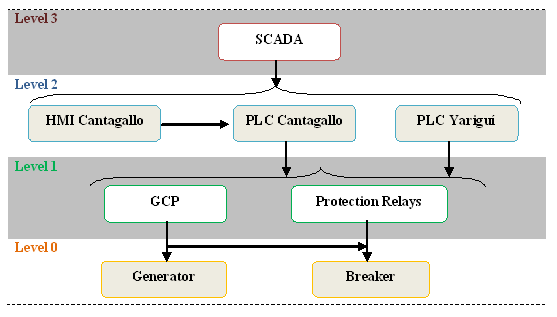
\includegraphics[width=0.5\textwidth]{img/sas.png}
  \caption{Hierarchical structure for the SAS}
  \label{fig:sas}
\end{figure}

\Fig{fig:sas} shows the suggested hierarchical control structure for
generation plants. This has a distributed configuration where hardware
and software are totally integrated to the main communication channel.

In the suggested solution an Ethernet network serves as core for all
the communications, with an 8 ports 100BaseTX switch. Because of the
location conditions broad band Radios were made available. These radios 
were set up in bridge mode using the IEEE 802.11 standard in the 2.46GHz 
band in order to do the remote link between the central control unit at
Yariguí and the electrical substation at Cantagallo. In this way the SAS
creates a virtual single information network in order to share data.
This can be seen in \fig{fig:arch} with the complete integrated solution.

\begin{figure*}
  \centering
  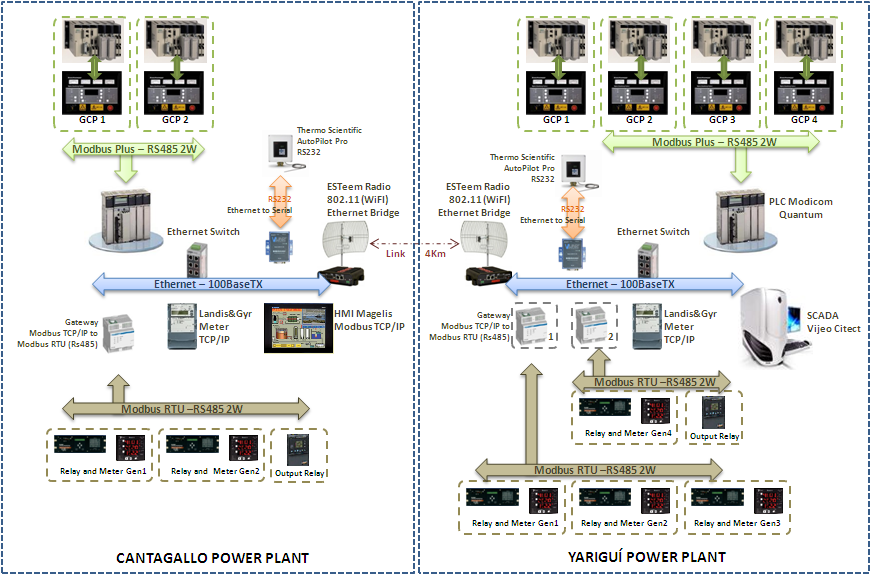
\includegraphics[width=1.0\textwidth]{img/arch.png}
  \caption{System architecture}
  \label{fig:arch}
\end{figure*}

A Modicon Quantum PLC stores data from the generators protection
relays, the output line's bay meters and the protection relay. The PLC
establishes the communication link with a Gateway trough the Modbus
TCP/IP protocol. This is translated to Modbus RTU (with a 2 wires
physical layer RS485) for data acquisition by each hardware that
corresponds to each bay.

At the Cantagallo generation center the Modbus RTU network has 5 nodes
deployed with one gateway. Likewise, the Yariguí generation center 
have two Gateways, one of them  with 6 nodes and the other with 3. 
This is done  in order to get fast data transfer and also for simplicity 
according to the hardware physical disposition.

The generators control units communication is done by the Modbus Plus
between the Quantum PLC and the Premium PLC included at the GCPs made
by Cummins. Only system supervision queries are run trough this bus.
The solution offers, in integrated control, the use of specific
Quantum PLC cards with digital outputs type contactor relay, digital inputs or
analog outputs related to the synchronization controls, start, stops,
trip signals, reset, generators parameters adjustment, etc.

The SCADA system used during the development is Vijeo Citect by
Schneider Electric. This integrates in a simple and fast way every
system communication because of the Modbus predominance with its
several versions installed at the generation center's hardware. The
SCADA operates on a DELL Server offering a stable and reliable
response for control and supervision.

Because the Cantagallo generation center must be remotely operated
an HMI was provided. From there, it is possible to send control
commands and full data supervision when local operation is required,
The HMI is a Magelis Smart tactile screen by the Schneider Electric 
manufacturer.

ThemoScientific gas meters use the Modbus Daniels protocol over a
serial RS232 interface. For this it was necessary to install on each
bus an Ethernet to serial (Serial Server) converter. This allows
multiple TCP connections on the same serial device. The converter
software emulates a virtual serial port enabling the SCADA to directly
consult the gas meter data.

The Landis \& Gyr meter is integrated to the Ethernet network by a
communication module offered by the manufacturer. Finally, The meter
data is collected and stored by the device software.

This way every electronic device within the generation centers is
integrated to the main communication network enabling an effective
solution with stable and reliable links.


%%-*-latex-*-

\section{Software}

\begin{figure}
  \centering
  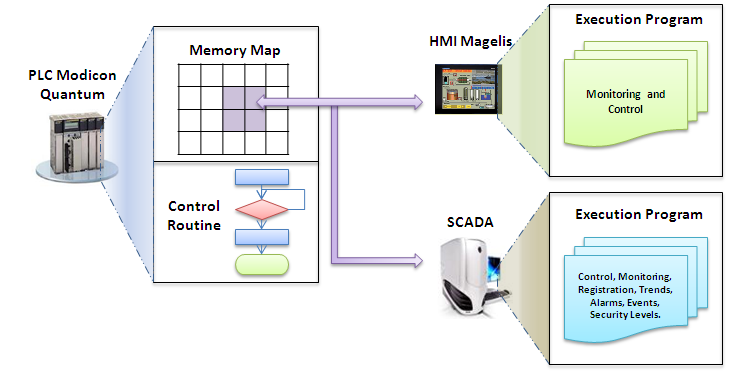
\includegraphics[width=0.5\textwidth]{img/software.png}
  \caption{Software interaction schema}
  \label{fig:software}
\end{figure}

The entire system development involved programming the Quantum PLC,
the HMI application and the SCADA software which is the automation's
main component. \Fig{fig:software} shows the schema of how the programs are
executed within each component. It is observed the interaction between
the PLC software trough a memory map used to read and write data
inside both the HMI and the SCADA. Intuitively, it is noted the
concept behind the automation system workings. Here, the SCADA or the
HMI writes a data at the PLC's memory map in order to execute a
command when a new control routine cycle begins.

\begin{figure}
  \centering
  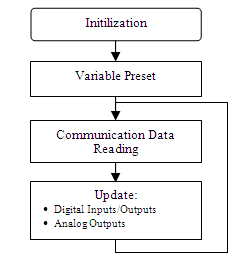
\includegraphics[width=0.2\textwidth]{img/plc.png}
  \caption{PLC routine blocks diagram}
  \label{fig:plc}
\end{figure}

The PLC software routine is developed at Ladder over Structured Text
because of its function within the system. The block diagram
represented by this routine is show in \fig{fig:plc}. In this diagram,
when the PLC begins the variables values are defined and preset. Immediately, the
reading of data is done trough the specified communication channels,
internally, the arithmetic operations for data conversion are also
executed and finally, the digital outputs and inputs and analog
outputs are updated. With this, a new operation cycle is started
obtaining a reliable execution and an efficient data update.

The Vijeo Designer software native to the Magelis Smart tactile
screens has been used for the programming of the HMI at the
Cantagallo generation center. The final application has interactive
menus to navigate, hardware control and supervision screens, security
access levels for users, tendencies graphs and a registry of active
and historic alarms. A  general view of the interface is shown in
\fig{fig:hmi}. For simplicity the operation of HMI is similar to the SCADA.

\begin{figure}
  \centering
  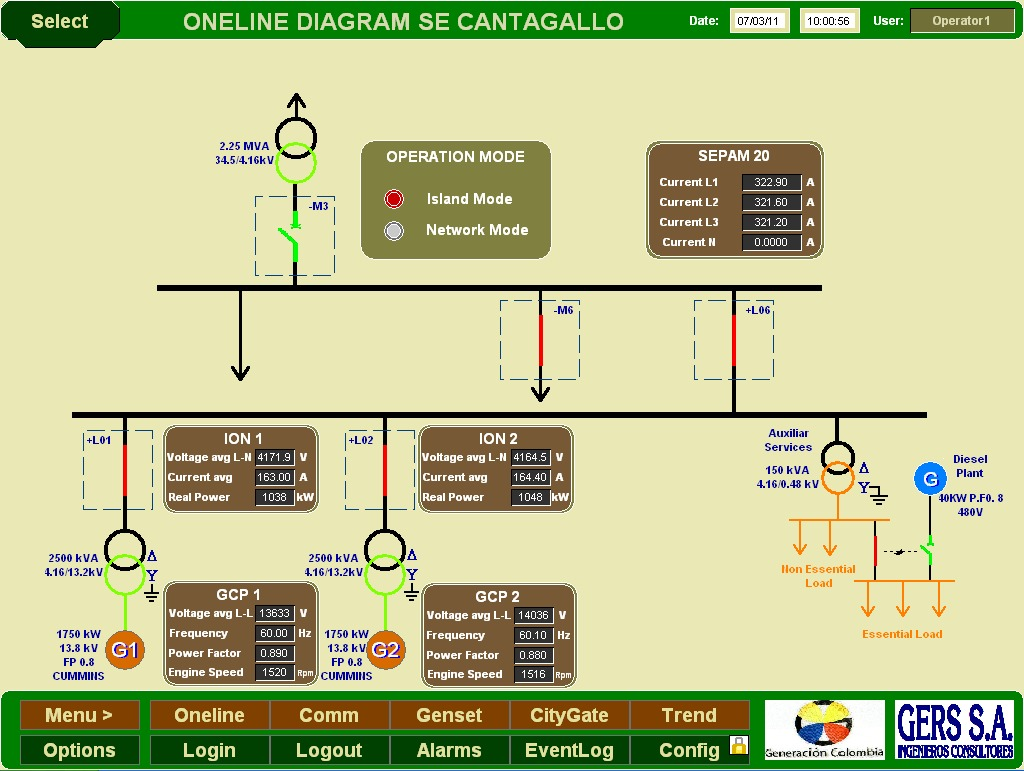
\includegraphics[width=0.5\textwidth]{img/hmi.png}
  \caption{Cantagallo Human-Machine Interface}
  \label{fig:hmi}
\end{figure}

The one-line diagram shows the HMI and the complete information
presented to the operator. Similarly the control schema are shown for
each generation bay and the supervision data are collected in a set of
screens for machines' electrical and mechanical data.

\begin{figure}
  \centering
  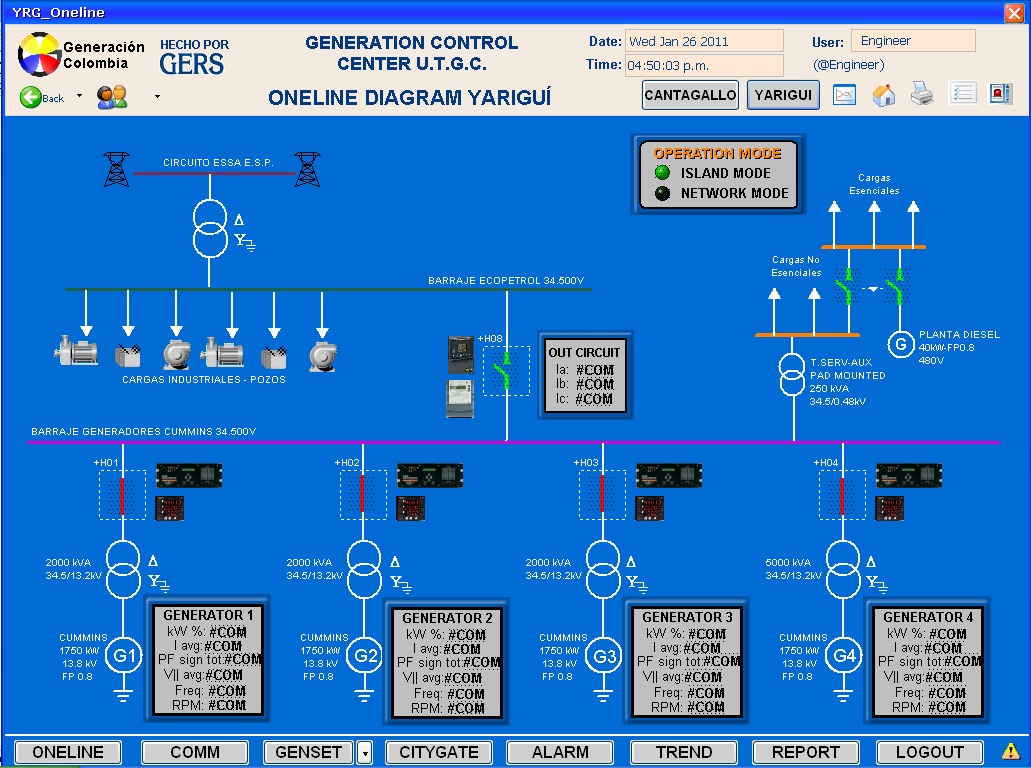
\includegraphics[width=0.5\textwidth]{img/oneline_scada.png}
  \caption{SCADA Vijeo Citect, Yariguí power plant one-line diagram}
  \label{fig:onelinescada}
\end{figure}

\begin{figure}
  \centering
  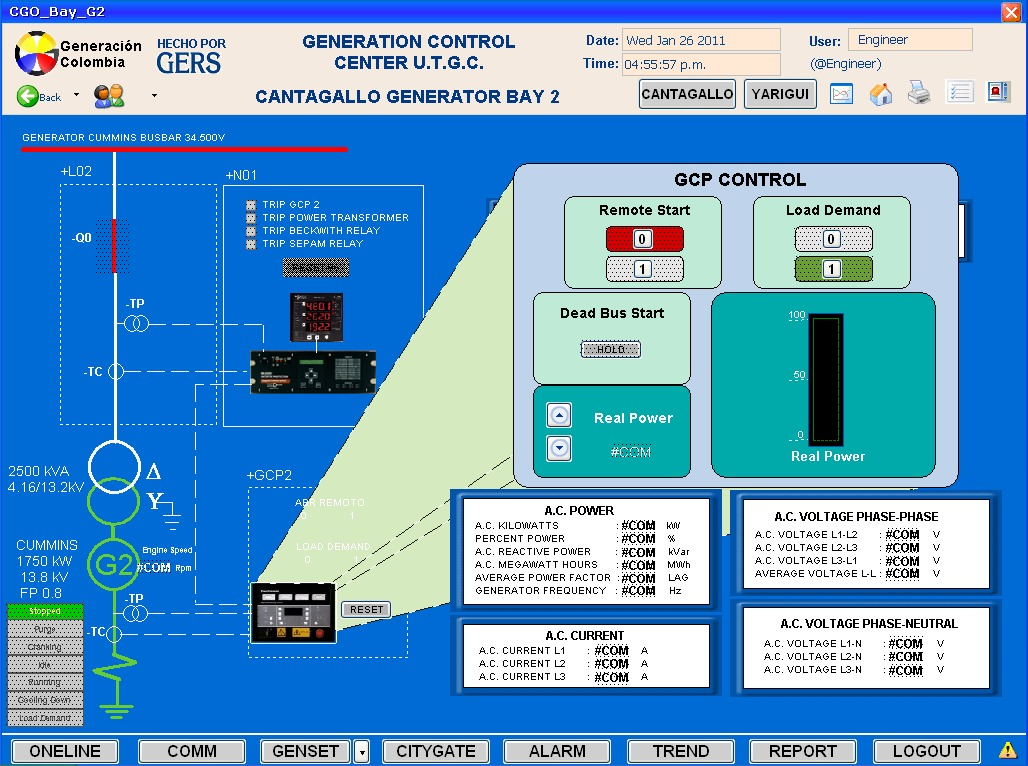
\includegraphics[width=0.5\textwidth]{img/bay_scada.png}
  \caption{SCADA Vijeo Citect, Control schema for Cantagallo power plant bay 2}
  \label{fig:bayscada}
\end{figure}

The characteristics programmed in the SCADA Vijeo Citect offer
supervision and control screens for each bay, besides of reports
generation, alarm informs, tendencies graphs, security records,
communication link status for damage reports. Every one of them
under the requirements initially expressed. \Fig{fig:onelinescada}
shows the running SCADA where the operation centers might be operated.

Bay control can be seen in \fig{fig:bayscada}, it offers every electrical
and mechanical data needed to operate the generators. They include:
start, stop, deadbus closure and the power variation given by the
generator during network mode (synchronization of the generation
center with the public electrical network). Additionally it shows the
reset for the several hardware in case of failure or trip and for the
synchronization of the generation centers with the network, the trip
in case of return to island mode and the opening and closing of the
output switch.

The gas meter data is integrated into the SCADA informing the operator
of the generator's gas input conditions. This functionality is vital
for being the gas the machine's combustible. The alarms screen has a
registry of active alarms, summarize and hardware alarms. Every alarm
has a priority level and a category used to generate a sound according
to the urgency. The tendencies screen offers to the operator the
capacity of viewing each variable of the generation center with data
store for as long as one year. It also offers ease of visualization
with capabilities like change of axis and scale. The following reports
can be generated: events, control operations made by every operator,
security access to the SCADA and a report of every alarm generated
during the previous year. Finally, security plays an important role on
every supervision and control system, to guarantee this, several access
levels have been created, including every system user such as operator,
engineer or administrator.

%%-*-latex-*-

\section{Running Tests}

The system running tests implies the verification of every supervision
data and the controls presents at the HMI and the developed SCADA.

As a supervision test schema a checklist was made including every
signal from every user interface. Every SCADA data signal returned
successful presenting an average update time of 1 second per data.

One important point is the communication link stability at Cantagallo
which proved the high efficiency during the supervision and control
tests.

An special display was created at the SCADA in order to monitor the
several communication networks available in the system. This shows both
a communication architecture at the generation center and the link state
for each device. Finally it helps to the maintenance and failure report
tasks.

Control tests executed and ordered for each generation center included
the tests for the HMI and the Cantagallo substation SCADA. The general
tests schema considered the following items:

\begin{itemize}
\item Control tests for each bay, including start, bar synchronization and stop.
\item Control tests for the output line interrupter: opening and closing.
\item Protection relays reset and interrupter shot sticking.
\item Re-synchronization with public network (generation center operation at
  network mode) transition to operation in Island mode and start of
  machines in dead bar.
\end{itemize}

The control signals were proved for each case altogether, resulting in effective
running and visualization tests.

Finally, at full operation, the Cantagallo-Yariguí communication channel
was supervised for a period of 24 hours. The results indicate that the
channel has an average packet loss rate of 1.0\%. Such results assure
the communications' stability.

%%-*-latex-*-

\section{Conclusion}

After the system was implemented and properly tested the following characteristics are emphasized:

\begin{itemize}
\item Entire stability and functionality of the Cantagallo generation
  center monitoring and remote control services. On account of the
  link stability and the conceived original design bringing both
  modularity and simplicity.
\item Human-machine interface gives the operator a simple control
  solution and a wide use of every device involved in the system.
\item We obtained an effective and easy to implement solution because of two
  factors. The first is the following of the guidelines of an ideal
  automation system architecture, with special focus on modularity and
  robustness. And the second is the integration of every equipment into
  the Ethernet communication main bus.
\item The effective implemented automation at the generation centers
  enables the supervision at each instant in order to support and
  diagnose the system.
\item System modularity and the acquired experience with the supply,
  installation, programming and the come into service of the generation
  centers automation ease the further development of similar works in
  the national territory.
\end{itemize}

\section*{Acknowledgement} Special thanks to all those who contributed on this development: Eduardo F. Caicedo, Luis E. Aragón, Juan M. Gers.

\bibliographystyle{IEEEtran}
\bibliography{IEEEabrv,automation}

\end{document}
